\section{Methodology}

HealthHub was developed through a phased approach, beginning with core infrastructure setup, followed by web development, AI integration, sensor system integration, and concluding with comprehensive testing. This structured timeline, illustrated in Figure \ref{fig:development-timeline}, ensured that each component was built and integrated systematically. The platform's architecture is designed to be modular and scalable, supporting a rich, interactive user experience focused on personal food safety and health monitoring.

\subsection{System Architecture}
HealthHub employs a multi-layered architecture, as depicted in Figure \ref{fig:system-architecture-overview}, to deliver its functionalities. 

\begin{figure}[!t]
\centering
\includegraphics[width=\columnwidth]{figures/hm-system-architecture.png}
\caption{Overview of HealthHub's System Architecture, showing frontend, backend, AI core, databases, and sensor connections.}
\label{fig:system-architecture-overview}
\end{figure}

\subsubsection{Frontend User Interface}
The user interacts with HealthHub through a responsive web application built with Next.js, React, and styled with Tailwind CSS. This interface allows users to log their daily food intake, view personalized health insights and nutritional summaries, and interact with an AI assistant via chat, voice, or video. The frontend is designed for intuitive navigation and clear presentation of complex food safety and health data.

\subsubsection{Backend Services}
User requests from the frontend are routed through an API Gateway to backend services. These services, developed using Node.js and Express, run within a scalable, auto-scaling Kubernetes cluster managed on AWS EC2 instances, with an Application Load Balancer distributing traffic. This robust backend handles business logic, data processing, and communication with other subsystems.

\subsubsection{AI Core: RAG and SQL Agents}
At the heart of HealthHub's intelligence is its AI core, implemented as a FastAPI service. This core comprises two main components orchestrated by LangChain:
\begin{itemize}
    \item \textbf{RAG Pipeline:} For answering food safety queries, HealthHub uses a RAG pipeline. This pipeline leverages powerful Large Language Models (LLMs like OpenAI's GPT series or Google's Gemini) and a Supabase Vector Database (pgvector). The database is populated with vectorized information from FSSAI documents, comprehensive food composition tables, allergen databases, and other relevant food safety literature. When a user asks a question, the RAG system retrieves the most relevant information chunks from the vector store to provide context for the LLM, which then generates an accurate and informative answer.
    \item \textbf{SQL Agent:} To analyze a user's logged dietary patterns, nutritional intake, and correlate this with sensor data, an SQL agent is employed. This agent converts natural language queries (either from the user or internal system triggers) into SQL commands to interact with the structured user data stored in the primary database.
\end{itemize}

\subsubsection{Data Management}
A Supabase SQL Database serves as the primary repository for user profile information, daily food logs, personal health metrics, and structured nutritional data. This database is queried by the SQL agent and provides historical context for personalized insights.

\subsubsection{Sensor Integration Subsystem}
To gather real-time physiological data, HealthHub integrates a wearable or nearby sensor array, the components of which are shown in Figure \ref{fig:sensor-components}, managed by an Arduino UNO R3 microcontroller. This unit interfaces with various sensors, including a MAX30102 for SpO2 and heart rate, an AD8232 for ECG data, an LM35 for body temperature, and a SEN-11574 pulse sensor. An ESP8266 Wi-Fi module facilitates wireless communication, transmitting the collected sensor data to the backend for storage and real-time analysis by the SQL agent and AI core. This allows HealthHub to potentially identify correlations between food intake and physiological changes, forming the basis for alerts.

\begin{figure}[!t]
\centering
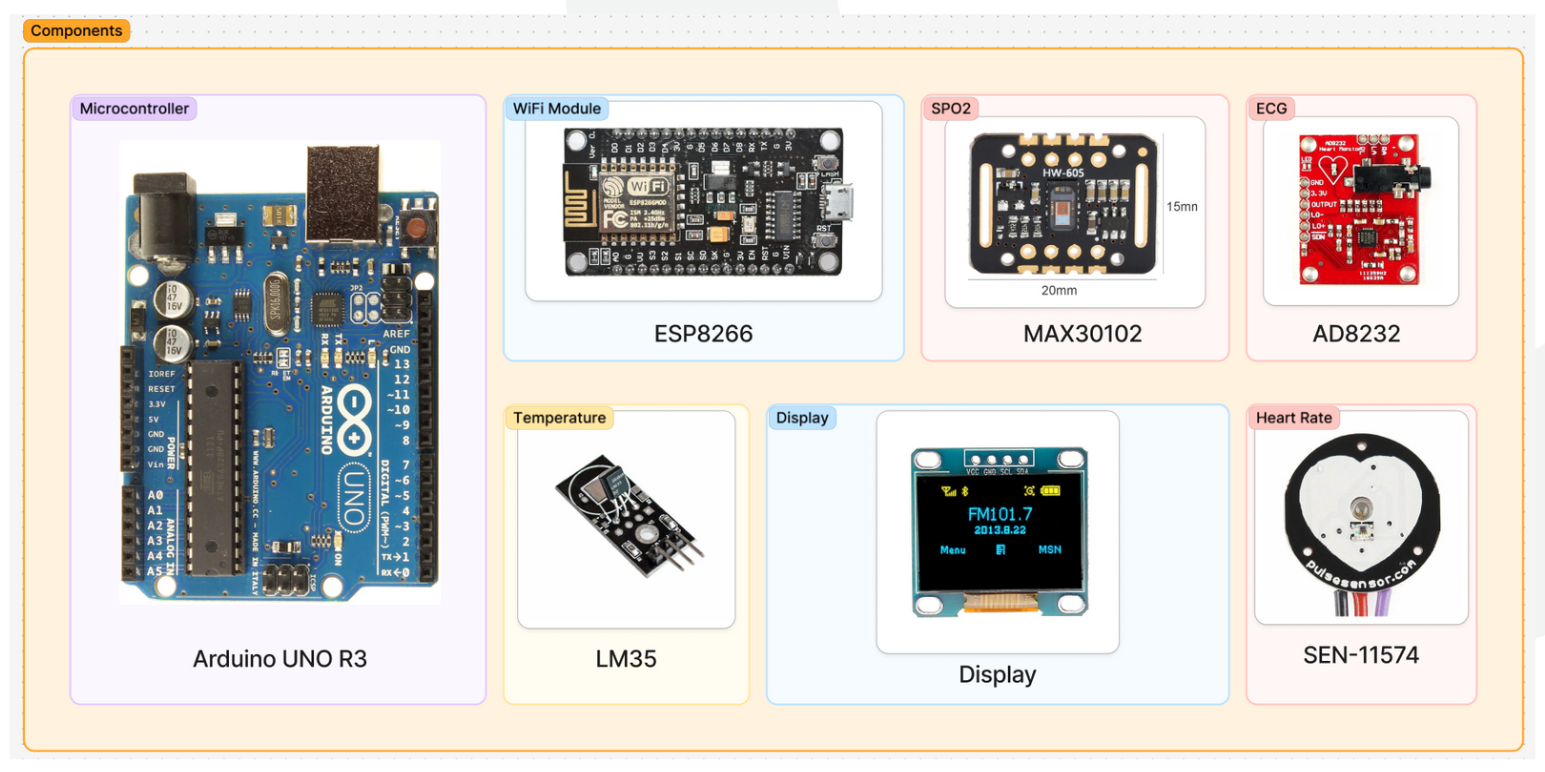
\includegraphics[width=\columnwidth]{figures/hm-sensors.png}
\caption{Key hardware components of the HealthHub sensor integration subsystem, including the Arduino UNO R3 microcontroller and various physiological sensors.}
\label{fig:sensor-components}
\end{figure}

\begin{figure}[!t]
\centering
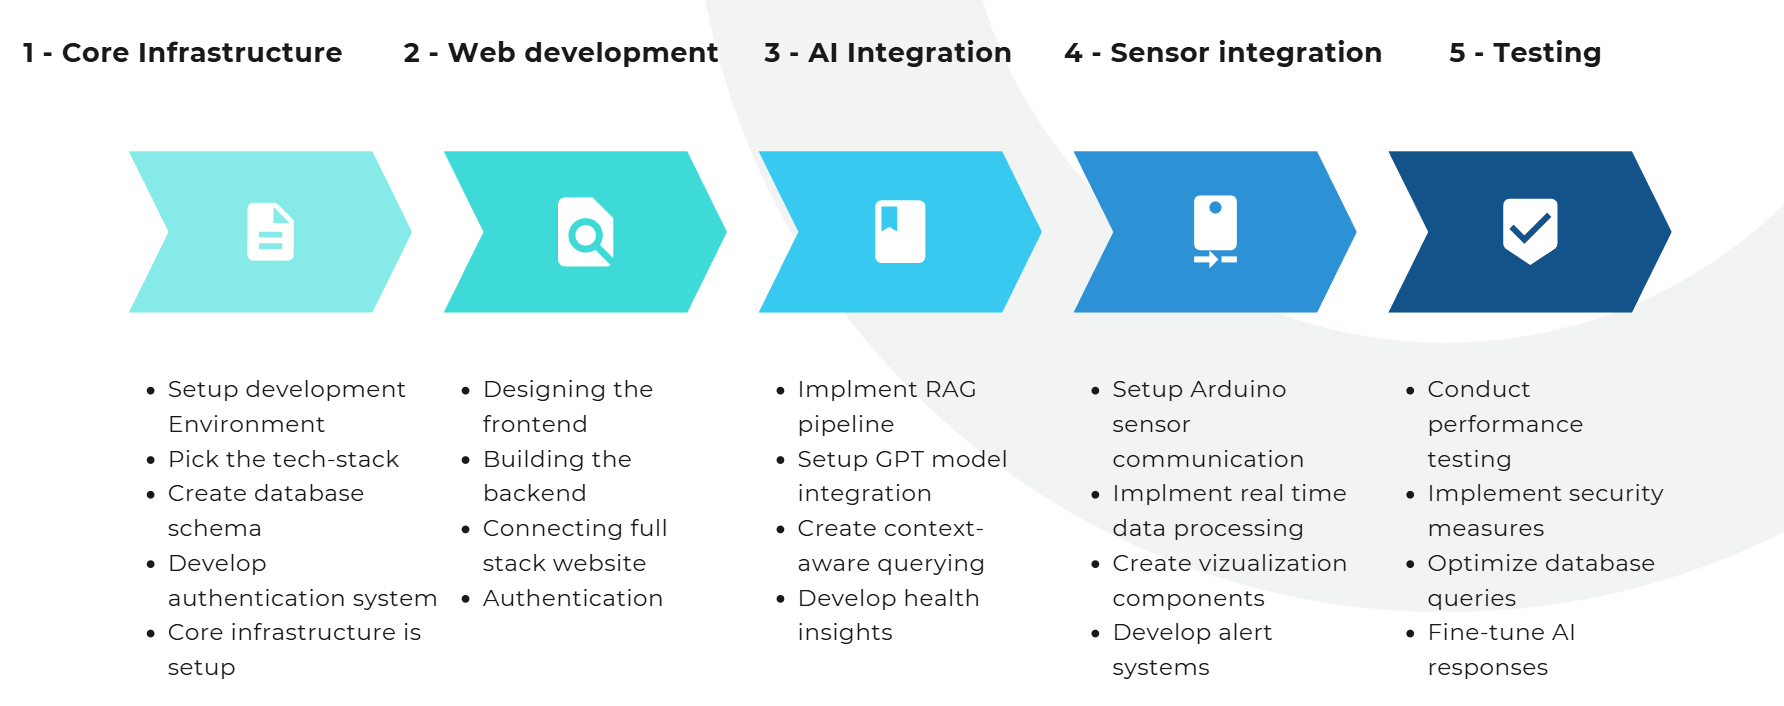
\includegraphics[width=\columnwidth]{figures/hm-timeline.png}
\caption{HealthHub Development Phases and Timeline.}
\label{fig:development-timeline}
\end{figure}

\subsection{HealthHub Workflow and User Interaction}
The typical user journey with HealthHub involves several key steps, designed to be seamless and empowering:

\textbf{1. Onboarding and Data Input:} New users create a profile. They can then log their daily food consumption through simple text input in the web interface. Simultaneously, if connected, the sensor subsystem automatically collects physiological data like heart rate, SpO2, and temperature, which is periodically sent to the backend.

\textbf{2. Querying and Information Retrieval:}
Users can interact with the HealthHub AI assistant using chat, voice, or video. For example:
\begin{itemize}
    \item To understand food safety, a user might ask, \textit{"Is the packaged juice I had this morning compliant with FSSAI sugar content guidelines?"} or \textit{"What are common allergens in pasta dishes?"} The RAG pipeline processes these queries, consults its specialized knowledge base (including FSSAI data), and provides a detailed, context-aware answer.
    \item For nutritional insights, a user could ask, \textit{"Show my protein intake for the last week,"} or the system might internally trigger the SQL agent to analyze, for instance, if a user's sodium intake consistently exceeds recommended levels based on their logged food.
\end{itemize}

\textbf{3. Personalized Feedback and Alerts:}
Based on the integrated data, HealthHub provides feedback through its interface:
\begin{itemize}
    \item Direct answers to user queries are displayed in the chat or spoken by the voice assistant.
    \item Nutritional summaries and dietary goal tracking are presented on the user's dashboard.
    \item Crucially, HealthHub can generate alerts or advisories. For example, if a user logs a food item known to have a recent FSSAI recall, or if their sensor data shows a significant, unexplained heart rate increase shortly after consuming a particular new food item, the system can flag this for the user's attention. These alerts are designed to be informative and prompt further awareness or consultation if needed.
\end{itemize}

\subsection{Knowledge Base for Food Safety}
The RAG pipeline's effectiveness relies on a comprehensive and up-to-date knowledge base. This includes, but is not limited to, official FSSAI circulars, food standards documentation, nutrient composition databases, peer-reviewed articles on food science and nutrition, and publicly available allergen information. This data is processed, chunked, and vectorized for efficient retrieval by the RAG system. 